
\subsubsection{Overview}

The Referee Box (Refbox) is an external component build by Aachen University. This component controls, monitors, and evaluates the game during the Robocup. It communicates with robots of both teams and the MPS, attributes the points and manages the different phases of the game. To get more information, it is recommended to read the referee box manual located at \url{http://www.robocup-logistics.org/refbox}. To set up the Refbox, the file “config.yaml” should be modified. The most important part to change in this file is the IP addresses (cf. next figure). \\

\begin{figure}[!h]
\centering
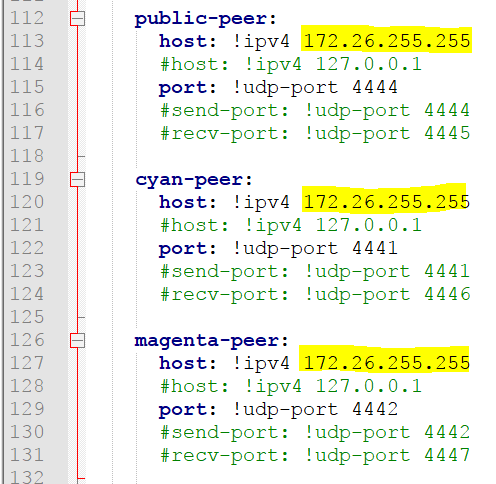
\includegraphics[]{pic/config_file_1.png}
\caption{Ip adresses to modify in config file}
\label{fig:configFile1}
\end{figure}

It is also needed to define a name for the team and a crypto key. It should be the same key in the Refbox server component.

\begin{figure}[!h]
\centering
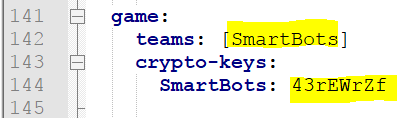
\includegraphics[]{pic/config_file_2.png}
\caption{Name and key to modify in config file}
\label{fig:configFile2}
\end{figure}

To run the Refbox, two programs should be executed in the same time: the main program (llsf-refbox) and the graphical interface (llsf-refbox-shell).

\begin{figure}[!h]
\centering
\includegraphics[width=\linewidth]{pic/graphical_refbox.png}
\caption{Graphical interface of the Refbox during Robocup 2017}
\label{fig:graphicalRefbox}
\end{figure}

\subsubsection{Situation in 2016}

There was no permanent Refbox installed in the laboratory. Each team was forced to install on a PC in the lab or on his own computer a Refbox with all necessary libraries. \\


\subsubsection{Situation in 2017}

During this year, a permanent Refbox with all the necessary libraries for the Robocup 2017 version (tneumann/rcll17) have been installed on an independent laptop. Any person that needs to test situations with the Refbox can take easily the laptop near his computer or access with XTightVncViewer.  To do this, it is necessary to run the server on the laptop with the command “tightvncserver”. Then it is possible to access with the command “xtightvncviewer <<ipAdress>> :1”.  In the current network, the IP address was “172.26.1.112”.
A window will be open and an access to the Refbox is possible (cf. next figure).\\

\begin{figure}[!h]
\centering
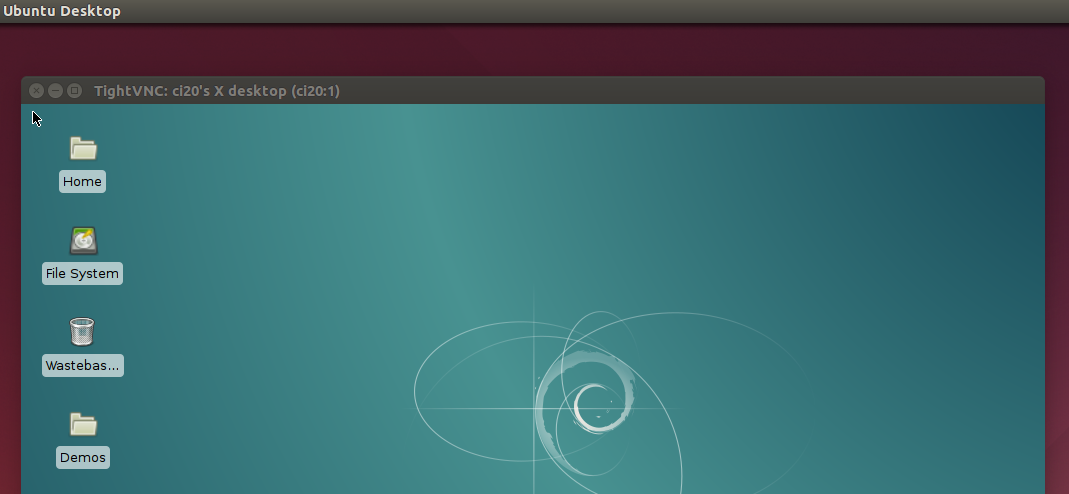
\includegraphics[width=\linewidth]{pic/xtightvncviewer.png}
\caption{Remote access to the Refbox laptop with XTightVncViewer}
\label{fig:xtightvncviewer}
\end{figure}

The Refbox changes regularly so it is necessary to update each new stable version of the Refbox. All versions can be found at this link: \url{https://git.fawkesrobotics.org/llsf-refbox.git}. A contact with Tim Niemueller \cite{RCLL2017}, one of the main developers of the Refbox, should be established to know the good (latest) version. \\


\subsubsection{Difficulties}

During the Robocup 2017, some difficulties have been faced. First, it is not possible to choose a zone for a MPS with the Refbox. It results that a successful test is more difficult to do in a smaller area. With this problem, we have used only check if the Refbox can detect the MPS report from Robotinos. We were not interested by a correct report. Indeed, there are not MPS in the center of the field with the current generation done by the Refbox. Another problem was to get the last version of the Refbox. Indeed, the current version in the trunk during the Robocup was the Refbox 2016. It was needed to search in the git repository to find the correct version of the Refbox. The last point was that the setting of the network was not easy during the Robocup. The Refbox is only useful during the test. Indeed, the official Refbox is used during the competition. The "test" Refbox should be identical to the official Refbox with the same crypto key to have quick change. \\
